\documentclass{article}

\def \lastexercisenumber {20}

% ---------------------------------------------------------------- %
% short package descriptions are copied from
% https://ctan.org/

% ---------------------------------------------------------------- %

% Accept different input encodings
\usepackage[utf8]{inputenc}

% Standard package for selecting font encodings
\usepackage[T1]{fontenc}

% ---------------------------------------------------------------- %

% Multilingual support for Plain TEX or LATEX
\usepackage[ngerman]{babel}

% ---------------------------------------------------------------- %

% Set all page margins to 1.5cm
\usepackage{fullpage}

% Margin adjustment and detection of odd/even pages
\usepackage{changepage}

% Flexible and complete interface to document dimensions
\usepackage{geometry}

% ---------------------------------------------------------------- %
% mathematics

\usepackage{amsmath}  % AMS mathematical facilities for LATEX
\usepackage{amssymb}
\usepackage{amsfonts} % TEX fonts from the American Mathematical Society
\usepackage{amsthm}   % Typesetting theorems (AMS style)

% Mathematical tools to use with amsmath
\usepackage{mathtools}

% Support for using RSFS fonts in maths
\usepackage{mathrsfs}

% Commands to produce dots in math that respect font size
\usepackage{mathdots}

% "Blackboard-style" cm fonts
\usepackage{bbm}

% Typeset in-line fractions in a "nice" way
\usepackage{nicefrac}

% Typeset quotient structures with LATEX
\usepackage{faktor}

% Vector arrows
\usepackage{esvect}

% St Mary Road symbols for theoretical computer science
\usepackage{stmaryrd}

% Three series of mathematical symbols
\usepackage{mathabx}

% ---------------------------------------------------------------- %
% algorithms

% Package for typesetting pseudocode
\usepackage{algpseudocode}

% Typeset source code listings using LATEX
\usepackage{listings}

% Reimplementation of and extensions to LATEX verbatim
\usepackage{verbatim}

% If necessary, please use the following 2 packages locally, but never both.
% This is because the algorithm environment gets defined in both packages, which leads to name conflicts.
% \usepackage{algorithm2e}
% \usepackage{algorithm}

% ---------------------------------------------------------------- %
% utilities

% A generic document command parser
\usepackage{xparse}

% Extended conditional commands
\usepackage{xifthen}

% e-TEX tools for LATEX
\usepackage{etoolbox}

% Define commands with suffixes
\usepackage{suffix}

% Extensive support for hypertext in LATEX
\usepackage{hyperref}

% Driver-independent color extensions for LATEX and pdfLATEX
\usepackage{xcolor}

% ---------------------------------------------------------------- %
% graphics

% -------------------------------- %

\usepackage{tikz}

% MISC
\usetikzlibrary{patterns}
\usetikzlibrary{decorations.markings}
\usetikzlibrary{positioning}
\usetikzlibrary{arrows}
\usetikzlibrary{arrows.meta}
\usetikzlibrary{overlay-beamer-styles}

% finite state machines
\usetikzlibrary{automata}

% turing machines
\usetikzlibrary{calc}
\usetikzlibrary{chains}
\usetikzlibrary{decorations.pathmorphing}

% -------------------------------- %

% Draw tree structures
\usepackage[noeepic]{qtree}

% Enhanced support for graphics
\usepackage{graphicx}

% Figures broken into subfigures
\usepackage{subfig}

% Improved interface for floating objects
\usepackage{float}

% Control float placement
\usepackage{placeins}

% Include PDF documents in LATEX
\usepackage{pdfpages}

% ---------------------------------------------------------------- %

% Control layout of itemize, enumerate, description
\usepackage[inline]{enumitem}

% Intermix single and multiple columns
\usepackage{multicol}
\setlength{\columnsep}{1cm}

% Coloured boxes, for LATEX examples and theorems, etc
\usepackage{tcolorbox}

% ---------------------------------------------------------------- %
% tables

% Tabulars with adjustable-width columns
\usepackage{tabularx}

% Tabular column heads and multilined cells
\usepackage{makecell}

% Publication quality tables in LATEX
\usepackage{booktabs}

% ---------------------------------------------------------------- %
% bibliography and quoting

% Sophisticated Bibliographies in LATEX
\usepackage[backend = biber, style = alphabetic]{biblatex}

% Context sensitive quotation facilities
\usepackage{csquotes}

% ---------------------------------------------------------------- %

% ---------------------------------------------------------------- %
% special letters

\newcommand{\N}{\mathbb N}
\newcommand{\Z}{\mathbb Z}
\newcommand{\Q}{\mathbb Q}
\newcommand{\R}{\mathbb R}
\newcommand{\C}{\mathbb C}
\newcommand{\K}{\mathbb K}
\newcommand{\T}{\mathbb T}
\newcommand{\E}{\mathbb E}
\newcommand{\V}{\mathbb V}
\renewcommand{\S}{\mathbb S}
\renewcommand{\P}{\mathbb P}
\newcommand{\1}{\mathbbm 1}
\newcommand{\G}{\mathbb G}

\newcommand{\iu}{\mathrm i}

% ---------------------------------------------------------------- %
% quantors

\newcommand{\Forall}        {\forall ~}
\newcommand{\Exists}        {\exists ~}
\newcommand{\nExists}       {\nexists ~}
\newcommand{\ExistsOnlyOne} {\exists! ~}
\newcommand{\nExistsOnlyOne}{\nexists! ~}
\newcommand{\ForAlmostAll}  {\forall^\infty ~}

% ---------------------------------------------------------------- %
% graphics boxed

\newcommand
{\includegraphicsboxed}
[2][0.75]
{
    \begin{center}
        \begin{tcolorbox}[standard jigsaw, opacityback = 0]

            \centering
            \includegraphics[width = #1 \textwidth]{#2}

        \end{tcolorbox}
    \end{center}
}

\newcommand
{\includegraphicsunboxed}
[2][0.75]
{
    \begin{center}
        \includegraphics[width = #1 \textwidth]{#2}
    \end{center}
}

\NewDocumentCommand
{\includegraphicsgraphicsboxed}
{ O{0.75} O{0.25} m m}
{
    \begin{center}
        \begin{tcolorbox}[standard jigsaw, opacityback = 0]

            \centering
            \includegraphics[width = #1 \textwidth]{#3} \\
            \vspace{#2 cm}
            \includegraphics[width = #1 \textwidth]{#4}

        \end{tcolorbox}
    \end{center}
}

\NewDocumentCommand
{\includegraphicsgraphicsunboxed}
{ O{0.75} O{0.25} m m}
{
    \begin{center}

        \centering
        \includegraphics[width = #1 \textwidth]{#3} \\
        \vspace{#2 cm}
        \includegraphics[width = #1 \textwidth]{#4}

    \end{center}
}

% ---------------------------------------------------------------- %
% braces

\newcommand{\pbraces}[1]{{\left  ( #1 \right  )}}
\newcommand{\bbraces}[1]{{\left  [ #1 \right  ]}}
\newcommand{\Bbraces}[1]{{\left \{ #1 \right \}}}
\newcommand{\vbraces}[1]{{\left  | #1 \right  |}}
\newcommand{\Vbraces}[1]{{\left \| #1 \right \|}}

\newcommand{\abraces}[1]{{\left \langle #1 \right \rangle}}

\newcommand{\floorbraces}[1]{{\left \lfloor #1 \right \rfloor}}
\newcommand{\ceilbraces} [1]{{\left \lceil  #1 \right \rceil }}

\newcommand{\dbbraces}    [1]{{\llbracket     #1 \rrbracket}}
\newcommand{\dpbraces}    [1]{{\llparenthesis #1 \rrparenthesis}}
\newcommand{\dfloorbraces}[1]{{\llfloor       #1 \rrfloor}}
\newcommand{\dceilbraces} [1]{{\llceil        #1 \rrceil}}

\newcommand{\dabraces}[1]{{\left \langle \left \langle #1 \right \rangle \right \rangle}}

\newcommand{\abs}  [1]{\vbraces{#1}}
\newcommand{\round}[1]{\bbraces{#1}}
\newcommand{\floor}[1]{\floorbraces{#1}}
\newcommand{\ceil} [1]{\ceilbraces{#1}}

% ---------------------------------------------------------------- %

% MISC

% metric spaces
\newcommand{\norm}[2][]{\Vbraces{#2}_{#1}}
\DeclareMathOperator{\metric}{d}
\DeclareMathOperator{\dist}  {dist}
\DeclareMathOperator{\diam}  {diam}

% O-notation
\newcommand{\landau}{{\scriptstyle \mathcal{O}}}
\newcommand{\Landau}{\mathcal{O}}

% ---------------------------------------------------------------- %

% math operators

% hyperbolic trigonometric function inverses
\DeclareMathOperator{\areasinh}{areasinh}
\DeclareMathOperator{\areacosh}{areacosh}
\DeclareMathOperator{\areatanh}{areatanh}

% special functions
\DeclareMathOperator{\id} {id}
\DeclareMathOperator{\sgn}{sgn}
\DeclareMathOperator{\Inv}{Inv}
\DeclareMathOperator{\erf}{erf}
\DeclareMathOperator{\pv} {pv}

% exponential function as power
\WithSuffix \newcommand \exp* [1]{\mathrm{e}^{#1}}

% operations on sets
\DeclareMathOperator{\meas}{meas}
\DeclareMathOperator{\card}{card}
\DeclareMathOperator{\Span}{span}
\DeclareMathOperator{\conv}{conv}
\DeclareMathOperator{\cof}{cof}
\DeclareMathOperator{\mean}{mean}
\DeclareMathOperator{\avg}{avg}
\DeclareMathOperator*{\argmax}{argmax}
\DeclareMathOperator*{\argsmax}{argsmax}

% number theory stuff
\DeclareMathOperator{\ggT}{ggT}
\DeclareMathOperator{\kgV}{kgV}
\DeclareMathOperator{\modulo}{mod}

% polynomial stuff
\DeclareMathOperator{\ord}{ord}
\DeclareMathOperator{\grad}{grad}

% function properties
\DeclareMathOperator{\ran}{ran}
\DeclareMathOperator{\supp}{supp}
\DeclareMathOperator{\graph}{graph}
\DeclareMathOperator{\dom}{dom}
\DeclareMathOperator{\Def}{def}
\DeclareMathOperator{\rg}{rg}

% matrix stuff
\DeclareMathOperator{\GL}{GL}
\DeclareMathOperator{\SL}{SL}
\DeclareMathOperator{\U}{U}
\DeclareMathOperator{\SU}{SU}
\DeclareMathOperator{\PSU}{PSU}
% \DeclareMathOperator{\O}{O}
% \DeclareMathOperator{\PO}{PO}
% \DeclareMathOperator{\PSO}{PSO}
\DeclareMathOperator{\diag}{diag}

% algebra stuff
\DeclareMathOperator{\At}{At}
\DeclareMathOperator{\Ob}{Ob}
\DeclareMathOperator{\Hom}{Hom}
\DeclareMathOperator{\End}{End}
\DeclareMathOperator{\Aut}{Aut}
\DeclareMathOperator{\Lin}{L}

% other function classes
\DeclareMathOperator{\Lip}{Lip}
\DeclareMathOperator{\Mod}{Mod}
\DeclareMathOperator{\Dil}{Dil}

% constants
\DeclareMathOperator{\NIL}{NIL}
\DeclareMathOperator{\eps}{eps}

% ---------------------------------------------------------------- %
% doubble & tripple powers

\newcommand
{\primeprime}
{{\prime \prime}}

\newcommand
{\primeprimeprime}
{{\prime \prime \prime}}

\newcommand
{\astast}
{{\ast \ast}}

\newcommand
{\astastast}
{{\ast \ast \ast}}

% ---------------------------------------------------------------- %
% derivatives

\NewDocumentCommand
{\derivative}
{ O{} O{} m m}
{
    \frac
    {\mathrm d^{#2} {#1}}
    {\mathrm d {#3}^{#2}}
}

\NewDocumentCommand
{\pderivative}
{ O{} O{} m m}
{
    \frac
    {\partial^{#2} {#1}}
    {\partial {#3}^{#2}}
}

\DeclareMathOperator{\Div}{div}
\DeclareMathOperator{\rot}{rot}

% ---------------------------------------------------------------- %
% integrals

\NewDocumentCommand
{\Int}
{ O{} O{} m m}
{\int_{#1}^{#2} #3 ~ \mathrm d #4}

\NewDocumentCommand
{\Iint}
{ O{} O{} m m m}
{\iint_{#1}^{#2} #3 ~ \mathrm d #4 ~ \mathrm d #5}

\NewDocumentCommand
{\Iiint}
{ O{} O{} m m m m}
{\iiint_{#1}^{#2} #3 ~ \mathrm d #4 ~ \mathrm d #5 ~ \mathrm d #6}

\NewDocumentCommand
{\Iiiint}
{ O{} O{} m m m m m}
{\iiiint_{#1}^{#2} #3 ~ \mathrm d #4 ~ \mathrm d #5 ~ \mathrm d #6 ~ \mathrm d #7}

\NewDocumentCommand
{\Idotsint}
{ O{} O{} m m m}
{\idotsint_{#1}^{#2} #3 ~ \mathrm d #4 \dots ~ \mathrm d #5}

\NewDocumentCommand
{\Oint}
{ O{} O{} m m}
{\oint_{#1}^{#2} #3 ~ \mathrm d #4}

% ---------------------------------------------------------------- %

% source:
% https://tex.stackexchange.com/questions/203257/tikz-chains-with-one-side-of-the-leftmost-node-thickbold

% #1 (optional): current state, e.g. $q_0$
% #2: cursor position, e.g. 1
% #3: number of displayed cells, e.g. 5
% #4: contents of cells, e.g. {$\triangleright$, $x_1$, \dots, $x_n$, \textvisiblespace}

\newcommand{\turingtape}[4][]
{
    \begin{tikzpicture}

        \tikzset{tape/.style={minimum size=.7cm, draw}}

        \begin{scope}[start chain=0 going right, node distance=0mm]
            \foreach \x [count=\i] in #4
            {
                \ifnum\i=#3 % if last node reset outer sep to 0pt
                    \node [on chain=0, tape, outer sep=0pt] (n\i) {\x};
                    \draw (n\i.north east) -- ++(.1,0) decorate [decoration={zigzag, segment length=.12cm, amplitude=.02cm}] {-- ($(n\i.south east)+(+.1,0)$)} -- (n\i.south east) -- cycle;
                \else
                    \node [on chain=0, tape] (n\i) {\x};
                \fi

                \ifnum\i=1 % if first node draw a thick line at the left
                    \draw [line width=.1cm] (n\i.north west) -- (n\i.south west);
                \fi
            }
 
            \node [right=.25cm of n#3] {$\cdots$};
            \node [tape, above left=.25cm and 1cm of n1] (q) {#1};
            \draw [>=latex, ->] (q) -| (n#2);

        \end{scope}

    \end{tikzpicture}
}

% ---------------------------------------------------------------- %

% ---------------------------------------------------------------- %
% amsthm-environments:

\theoremstyle{definition}

% numbered theorems
\newtheorem{theorem}             {Satz}[section]
\newtheorem{lemma}      [theorem]{Lemma}
\newtheorem{corollary}  [theorem]{Korollar}
\newtheorem{proposition}[theorem]{Proposition}
\newtheorem{remark}     [theorem]{Bemerkung}
\newtheorem{definition} [theorem]{Definition}
\newtheorem{example}    [theorem]{Beispiel}
\newtheorem{heuristics} [theorem]{Heuristik}

% unnumbered theorems
\newtheorem*{theorem*}    {Satz}
\newtheorem*{lemma*}      {Lemma}
\newtheorem*{corollary*}  {Korollar}
\newtheorem*{proposition*}{Proposition}
\newtheorem*{remark*}     {Bemerkung}
\newtheorem*{definition*} {Definition}
\newtheorem*{example*}    {Beispiel}
\newtheorem*{heuristics*} {Heuristik}

% ---------------------------------------------------------------- %
% exercise- and solution-environments:

% Please define this stuff in project ("main.tex"):
% \def \lastexercisenumber {...}

\newtheorem{exercise}{Aufgabe}
\setcounter{exercise}{\lastexercisenumber}

\newenvironment{solution}
{
  \begin{proof}[Lösung]
}{
  \end{proof}
}

% ---------------------------------------------------------------- %
% MISC translations for environment-names

\renewcommand{\proofname} {Beweis}
\renewcommand{\figurename}{Abbildung}
\renewcommand{\tablename} {Tabelle}

% ---------------------------------------------------------------- %

% ---------------------------------------------------------------- %
% https://www.overleaf.com/learn/latex/Code_listing

\definecolor{codegreen} {rgb}{0, 0.6, 0}
\definecolor{codegray}    {rgb}{0.5, 0.5, 0.5}
\definecolor{codepurple}{rgb}{0.58, 0, 0.82}
\definecolor{backcolour}{rgb}{0.95, 0.95, 0.92}

\lstdefinestyle{overleaf}
{
    backgroundcolor = \color{backcolour},
    commentstyle = \color{codegreen},
    keywordstyle = \color{magenta},
    numberstyle = \tiny\color{codegray},
    stringstyle = \color{codepurple},
    basicstyle = \ttfamily \footnotesize,
    breakatwhitespace = false,
    breaklines = true,
    captionpos = b,
    keepspaces = true,
    numbers = left,
    numbersep = 5pt,
    showspaces = false,
    showstringspaces = false,
    showtabs = false,
    tabsize = 2
}

% ---------------------------------------------------------------- %
% https://en.wikibooks.org/wiki/LaTeX/Source_Code_Listings

\lstdefinestyle{customc}
{
    belowcaptionskip = 1 \baselineskip,
    breaklines = true,
    frame = L,
    xleftmargin = \parindent,
    language = C,
    showstringspaces = false,
    basicstyle = \footnotesize \ttfamily,
    keywordstyle = \bfseries \color{green!40!black},
    commentstyle = \itshape \color{purple!40!black},
    identifierstyle = \color{blue},
    stringstyle = \color{orange},
}

\lstdefinestyle{customasm}
{
    belowcaptionskip = 1 \baselineskip,
    frame = L,
    xleftmargin = \parindent,
    language = [x86masm] Assembler,
    basicstyle = \footnotesize\ttfamily,
    commentstyle = \itshape\color{purple!40!black},
}

% ---------------------------------------------------------------- %
% https://tex.stackexchange.com/questions/235731/listings-syntax-for-literate

\definecolor{maroon}        {cmyk}{0, 0.87, 0.68, 0.32}
\definecolor{halfgray}      {gray}{0.55}
\definecolor{ipython_frame} {RGB}{207, 207, 207}
\definecolor{ipython_bg}    {RGB}{247, 247, 247}
\definecolor{ipython_red}   {RGB}{186, 33, 33}
\definecolor{ipython_green} {RGB}{0, 128, 0}
\definecolor{ipython_cyan}  {RGB}{64, 128, 128}
\definecolor{ipython_purple}{RGB}{170, 34, 255}

\lstdefinestyle{stackexchangePython}
{
    breaklines = true,
    %
    extendedchars = true,
    literate =
    {á}{{\' a}} 1 {é}{{\' e}} 1 {í}{{\' i}} 1 {ó}{{\' o}} 1 {ú}{{\' u}} 1
    {Á}{{\' A}} 1 {É}{{\' E}} 1 {Í}{{\' I}} 1 {Ó}{{\' O}} 1 {Ú}{{\' U}} 1
    {à}{{\` a}} 1 {è}{{\` e}} 1 {ì}{{\` i}} 1 {ò}{{\` o}} 1 {ù}{{\` u}} 1
    {À}{{\` A}} 1 {È}{{\' E}} 1 {Ì}{{\` I}} 1 {Ò}{{\` O}} 1 {Ù}{{\` U}} 1
    {ä}{{\" a}} 1 {ë}{{\" e}} 1 {ï}{{\" i}} 1 {ö}{{\" o}} 1 {ü}{{\" u}} 1
    {Ä}{{\" A}} 1 {Ë}{{\" E}} 1 {Ï}{{\" I}} 1 {Ö}{{\" O}} 1 {Ü}{{\" U}} 1
    {â}{{\^ a}} 1 {ê}{{\^ e}} 1 {î}{{\^ i}} 1 {ô}{{\^ o}} 1 {û}{{\^ u}} 1
    {Â}{{\^ A}} 1 {Ê}{{\^ E}} 1 {Î}{{\^ I}} 1 {Ô}{{\^ O}} 1 {Û}{{\^ U}} 1
    {œ}{{\oe}}  1 {Œ}{{\OE}}  1 {æ}{{\ae}}  1 {Æ}{{\AE}}  1 {ß}{{\ss}}  1
    {ç}{{\c c}} 1 {Ç}{{\c C}} 1 {ø}{{\o}} 1 {å}{{\r a}} 1 {Å}{{\r A}} 1
    {€}{{\EUR}} 1 {£}{{\pounds}} 1
}


% Python definition (c) 1998 Michael Weber
% Additional definitions (2013) Alexis Dimitriadis
% modified by me (should not have empty lines)

\lstdefinelanguage{iPython}{
    morekeywords = {access, and, break, class, continue, def, del, elif, else, except, exec, finally, for, from, global, if, import, in, is, lambda, not, or, pass, print, raise, return, try, while}, %
    %
    % Built-ins
    morekeywords = [2]{abs, all, any, basestring, bin, bool, bytearray, callable, chr, classmethod, cmp, compile, complex, delattr, dict, dir, divmod, enumerate, eval, execfile, file, filter, float, format, frozenset, getattr, globals, hasattr, hash, help, hex, id, input, int, isinstance, issubclass, iter, len, list, locals, long, map, max, memoryview, min, next, object, oct, open, ord, pow, property, range, raw_input, reduce, reload, repr, reversed, round, set, setattr, slice, sorted, staticmethod, str, sum, super, tuple, type, unichr, unicode, vars, xrange, zip, apply, buffer, coerce, intern}, %
    %
    sensitive = true, %
    morecomment = [l] \#, %
    morestring = [b]', %
    morestring = [b]", %
    %
    morestring = [s]{'''}{'''}, % used for documentation text (mulitiline strings)
    morestring = [s]{"""}{"""}, % added by Philipp Matthias Hahn
    %
    morestring = [s]{r'}{'},     % `raw' strings
    morestring = [s]{r"}{"},     %
    morestring = [s]{r'''}{'''}, %
    morestring = [s]{r"""}{"""}, %
    morestring = [s]{u'}{'},     % unicode strings
    morestring = [s]{u"}{"},     %
    morestring = [s]{u'''}{'''}, %
    morestring = [s]{u"""}{"""}, %
    %
    % {replace}{replacement}{lenght of replace}
    % *{-}{-}{1} will not replace in comments and so on
    literate = 
    {á}{{\' a}} 1 {é}{{\' e}} 1 {í}{{\' i}} 1 {ó}{{\' o}} 1 {ú}{{\' u}} 1
    {Á}{{\' A}} 1 {É}{{\' E}} 1 {Í}{{\' I}} 1 {Ó}{{\' O}} 1 {Ú}{{\' U}} 1
    {à}{{\` a}} 1 {è}{{\` e}} 1 {ì}{{\` i}} 1 {ò}{{\` o}} 1 {ù}{{\` u}} 1
    {À}{{\` A}} 1 {È}{{\' E}} 1 {Ì}{{\` I}} 1 {Ò}{{\` O}} 1 {Ù}{{\` U}} 1
    {ä}{{\" a}} 1 {ë}{{\" e}} 1 {ï}{{\" i}} 1 {ö}{{\" o}} 1 {ü}{{\" u}} 1
    {Ä}{{\" A}} 1 {Ë}{{\" E}} 1 {Ï}{{\" I}} 1 {Ö}{{\" O}} 1 {Ü}{{\" U}} 1
    {â}{{\^ a}} 1 {ê}{{\^ e}} 1 {î}{{\^ i}} 1 {ô}{{\^ o}} 1 {û}{{\^ u}} 1
    {Â}{{\^ A}} 1 {Ê}{{\^ E}} 1 {Î}{{\^ I}} 1 {Ô}{{\^ O}} 1 {Û}{{\^ U}} 1
    {œ}{{\oe}}  1 {Œ}{{\OE}}  1 {æ}{{\ae}}  1 {Æ}{{\AE}}  1 {ß}{{\ss}}  1
    {ç}{{\c c}} 1 {Ç}{{\c C}} 1 {ø}{{\o}} 1 {å}{{\r a}} 1 {Å}{{\r A}} 1
    {€}{{\EUR}} 1 {£}{{\pounds}} 1
    %
    {^}{{{\color{ipython_purple}\^ {}}}} 1
    { = }{{{\color{ipython_purple} = }}} 1
    %
    {+}{{{\color{ipython_purple}+}}} 1
    {*}{{{\color{ipython_purple}$^\ast$}}} 1
    {/}{{{\color{ipython_purple}/}}} 1
    %
    {+=}{{{+=}}} 1
    {-=}{{{-=}}} 1
    {*=}{{{$^\ast$ = }}} 1
    {/=}{{{/=}}} 1,
    literate = 
    *{-}{{{\color{ipython_purple} -}}} 1
     {?}{{{\color{ipython_purple} ?}}} 1,
    %
    identifierstyle = \color{black}\ttfamily,
    commentstyle = \color{ipython_cyan}\ttfamily,
    stringstyle = \color{ipython_red}\ttfamily,
    keepspaces = true,
    showspaces = false,
    showstringspaces = false,
    %
    rulecolor = \color{ipython_frame},
    frame = single,
    frameround = {t}{t}{t}{t},
    framexleftmargin = 6mm,
    numbers = left,
    numberstyle = \tiny\color{halfgray},
    %
    %
    backgroundcolor = \color{ipython_bg},
    % extendedchars = true,
    basicstyle = \scriptsize,
    keywordstyle = \color{ipython_green}\ttfamily,
}

% ---------------------------------------------------------------- %
% https://tex.stackexchange.com/questions/417884/colour-r-code-to-match-knitr-theme-using-listings-minted-or-other

\geometry{verbose, tmargin = 2.5cm, bmargin = 2.5cm, lmargin = 2.5cm, rmargin = 2.5cm}

\definecolor{backgroundCol}  {rgb}{.97, .97, .97}
\definecolor{commentstyleCol}{rgb}{0.678, 0.584, 0.686}
\definecolor{keywordstyleCol}{rgb}{0.737, 0.353, 0.396}
\definecolor{stringstyleCol} {rgb}{0.192, 0.494, 0.8}
\definecolor{NumCol}         {rgb}{0.686, 0.059, 0.569}
\definecolor{basicstyleCol}  {rgb}{0.345, 0.345, 0.345}

\lstdefinestyle{stackexchangeR}
{
    language = R,                                        % the language of the code
    basicstyle = \small \ttfamily \color{basicstyleCol}, % the size of the fonts that are used for the code
    % numbers = left,                                      % where to put the line-numbers
    numberstyle = \color{green},                         % the style that is used for the line-numbers
    stepnumber = 1,                                      % the step between two line-numbers. If it is 1, each line will be numbered
    numbersep = 5pt,                                     % how far the line-numbers are from the code
    backgroundcolor = \color{backgroundCol},             % choose the background color. You must add \usepackage{color}
    showspaces = false,                                  % show spaces adding particular underscores
    showstringspaces = false,                            % underline spaces within strings
    showtabs = false,                                    % show tabs within strings adding particular underscores
    % frame = single,                                      % adds a frame around the code
    % rulecolor = \color{white},                           % if not set, the frame-color may be changed on line-breaks within not-black text (e.g. commens (green here))
    tabsize = 2,                                         % sets default tabsize to 2 spaces
    captionpos = b,                                      % sets the caption-position to bottom
    breaklines = true,                                   % sets automatic line breaking
    breakatwhitespace = false,                           % sets if automatic breaks should only happen at whitespace
    keywordstyle = \color{keywordstyleCol},              % keyword style
    commentstyle = \color{commentstyleCol},              % comment style
    stringstyle = \color{stringstyleCol},                % string literal style
    literate = %
    *{0}{{{\color{NumCol} 0}}} 1
     {1}{{{\color{NumCol} 1}}} 1
     {2}{{{\color{NumCol} 2}}} 1
     {3}{{{\color{NumCol} 3}}} 1
     {4}{{{\color{NumCol} 4}}} 1
     {5}{{{\color{NumCol} 5}}} 1
     {6}{{{\color{NumCol} 6}}} 1
     {7}{{{\color{NumCol} 7}}} 1
     {8}{{{\color{NumCol} 8}}} 1
     {9}{{{\color{NumCol} 9}}} 1
}

% ---------------------------------------------------------------- %
% Fundament Mathematik

\lstdefinestyle{fundament}{basicstyle = \ttfamily}

% ---------------------------------------------------------------- %


\addbibresource{../../../Fundament-LaTeX/references.bib}

\graphicspath{{../../../Fundament-LaTeX/images/}}

\parskip 0pt
\parindent 0pt

\title
{
  Numerik von Partiellen Differentialgleichungen: stationäre Probleme \\
  \vspace{4pt}
  \normalsize
  \textit{5. Übung am 09.12.2020}
}
\author
{
  Richard Weiss
  \and
  Florian Schager
  \and
  Christian Sallinger
  %\and
  %Fabian Zehetgruber
  %\and
  %Paul Winkler
  %\and
  %Christian Göth
}
\date{}

\begin{document}

\maketitle

% --------------------------------------------------------------------------------

\begin{exercise}

Sei $A \in \R^{2 \times 2}$ eine symmetrische, positiv definite Matrix, $b \in \R^2$ und $c > 0$ mit $c - \frac{1}{2}\Div(b) \geq 0$.
Weiter seien $\Omega \subset \R^2$ ein beschränktes Lipschitz-Gebiet und $f \in L^2(\Omega)$.

\begin{enumerate}[label = \textbf{\alph*)}]

  \item Beweisen Sie, dass eine eindeutige schwache Lösung $u \in H_0^1(\Omega)$ von

  \begin{subequations}
    \begin{align}
      -\Div(A\nabla u) + b \cdot \nabla u + cu &= f \qquad \text{auf } \Omega, \label{eq:1A} \\
      u &= 0 \qquad \text{auf } \partial\Omega, \label{eq:1B}
    \end{align}
  \end{subequations}

  existiert.

  \item Sei $u_h \in \mathcal{S}_0^1(\mathcal{T})$ die eindeutige, schwache Finite-Elemente Lösung.
  Konstruieren Sie einen residualen Fehlerschätzer für
  $\norm[H_0^1(\Omega)]{u - u_h}$.

  \item Beweisen Sie, dass dieser Fehlerschätzer zuverlässig ist.

\end{enumerate}

\textit{Hinweis:}
Zeigen Sie zuerst, dass die zugehörige Bilinearform elliptisch ist.

\end{exercise}

% --------------------------------------------------------------------------------

\begin{solution}

Wir stellen zuerst das Funktional und die Bilinearform für die schwache Formlierung der PDE (1) auf.
$\Forall v \in H_0^1(\Omega):$

\begin{align*}
  F(v)
  & :=
  \Int[\Omega]{f v}{x}
  \stackrel{!}{=}
  \Int[\Omega]{(-\Div(A \nabla u) + b \cdot \nabla u + c u) v}{x}
  =
  -\Int[\Omega]{\Div(A \nabla u) v}{x}
  +
  \Int[\Omega]{(b \cdot \nabla u + c u) v}{x} \\
  & \stackrel
  {
    \mathrm{PI}
  }{=}
  \Int[\Omega]{A \nabla u \cdot \nabla v}
  -
  \underbrace
  {
    \Int[\partial \Omega]{(A \nabla u \cdot \nu) v}{s}
  }_0
  +
  \Int[\Omega]{(b \cdot \nabla u + c u) v}{x}
  =
  \Int[\Omega]{(\nabla u, \nabla v)_A + (b \cdot \nabla u + c u) v}{x} \\
  & =:
  a(u, v)
\end{align*}

Weil $\R^2$ endlich-dimensional ist, ist die, wegen der Symmetrie und positiven Definitheit von $A$ wohldefinierte, Energie-Norm $\norm[A]{\cdot}$ äquivalent zur Euklid-Norm $|\cdot|$.

\begin{align*}
  \implies
  \Exists \alpha, \beta > 0:
  \alpha |\cdot| \leq \norm[A]{\cdot} \leq \beta |\cdot|
\end{align*}

\begin{enumerate}[label = \textbf{\alph*)}]

  \item Wir wollen Exercise 7.2 (Lemma of Lax-Milgram) auf $F$ und $a$ anwenden.
  
  \begin{enumerate}[label = \arabic*.]

    \item $a$ stetig:
    
    \begin{align*}
      a(u, v)
      & =
      \Int[\Omega]{(\nabla u, \nabla v)_A + (b \cdot \nabla u + c u) v}{x}
      \stackrel
      {
        \mathrm{CSB}
      }{\leq}
      \Int[\Omega]{\norm[A]{\nabla u} \norm[A]{\nabla v} + |b| |\nabla u| v + c u v}{x} \\
      & \stackrel
      {
        \mathrm{CSB}
      }{\leq}
      \beta^2 \Int[\Omega]{|\nabla u| |\nabla v|}{x}
      +
      \norm[L^\infty]{b} \Int[\Omega]{|\nabla u| |v|}{x}
      +
      c \Int[\Omega]{u v}{x} \\
      & \leq
      \beta^2 \norm[L^2(\Omega)]{\nabla u} \norm[L^2(\Omega)]{\nabla v}
      +
      \norm[L^\infty(\Omega)]{b} \norm[L^2(\Omega)]{\nabla u} \norm[L^2(\Omega)]{v}
      +
      c \norm[L^2(\Omega)]{u} \norm[L^2(\Omega)]{v} \\
      & \leq
      \max \Bbraces{\beta^2, \norm[L^\infty(\Omega)]{b}, c} \norm[H^1(\Omega)]{u} \norm[H^1(\Omega)]{v}
    \end{align*}

    \item $a$ elliptisch:
    
    Die Produktregel für $\Div$ liefert uns
    
    \begin{align*}
      \Div(u^2 b) = \nabla(u^2) b + u^2 \Div b = 2 u b \nabla u + u^2 \Div b
      \implies
      u b \cdot \nabla u = \frac{1}{2} (\Div(u^2 b) - u \Div b),
    \end{align*}

    und der Integral-Satz von Gauß, dass ($u \in H_0^1(\Omega)$)

    \begin{align*}
      \Int[\Omega]{\Div (u^2 b)}{x}
      =
      \Int[\partial \Omega]{u^2 b \cdot \nu}{s}
      =
      0.
    \end{align*}

    Wir verwenden die Poincaré-Ungleichung.

    \includegraphicsboxed{PDEs/PDEs_-_Satz_5-11_(Poincare-Ungleichung).png}

    \begin{align*}
      \implies
      a(u, u)
      & =
      \Int[\Omega]{(\nabla u, \nabla u)_A + (b \cdot \nabla u + c u) v}{x}
      =
      \Int[\Omega]{\norm[A]{u}^2 + u b \cdot \nabla u + c u^2}{x} \\
      & \geq
      \Int[\Omega]{\alpha^2 |\nabla u|^2 + \frac{1}{2} (\Div(u^2 b) - u \Div b) + c u^2}{x} \\
      & =
      \alpha^2 \norm[L^2(\Omega)]{\nabla u}^2
      +
      \frac{1}{2} \Int[\partial \Omega]{u^2 b \cdot \nu}{s}
      +
      \underbrace
      {
        \Int[\Omega]{\pbraces{c - \frac{1}{2} \Div b} u^2}{x}
      }_{
        \geq 0
      } \\
      & \geq
      \alpha^2 \norm[L^2(\Omega)]{\nabla u}^2
      \geq
      \pbraces{\frac{\alpha}{C_P}}^2 \norm[H^1(\Omega)]{u}^2
    \end{align*}

  \end{enumerate}

  \item Siehe \textbf{c)} ...
  
  \item Wir formulieren ein Analogon zu Theorem 4.11.
  
  \includegraphicsboxed{NumPDEs/NumPDEs - Theorem 4.11.png}

  \begin{tcolorbox}[standard jigsaw, opacityback = 0]
    \textbf{Theorem 4.11. (Hier könnte Ihre Werbung stehen!)}
    Der Fehlerschätzer

    \begin{align*}
      \eta
      :=
      \pbraces
      {
        \norm[L^2(\Omega)]{h_\mathcal{T} (f - b \cdot \nabla u_h - c u_h)}^2
        +
        \norm[L^2(\mathcal{E}_\Omega)]{h_\mathcal{E}^{1/2} \dbbraces{\partial_n u_h}}^2
      }^{1/2}
    \end{align*}

    genügt der Zuverlässigkeits-Abschätzung

    \begin{align*}
      \norm[H^1(\Omega)]{u - u_h}
      \leq
      C \eta,
    \end{align*}

    wobei die Konstante $C > 0$ von der $\gamma$-Form-Regularität von $\mathcal{T}$ abhängt.

  \end{tcolorbox}

  \textbf{Beweis.}
  Für alle $w \in H_D^1(\Omega)$ und $T \in \mathcal{T}$, führt partielle Integration, und die Tatsache, dass $u_h \in \mathcal{S}^1(\Omega)$ und $A$ konstant ist, zu

  \begin{multline*}
    \Int[T]{(\nabla u_h, \nabla w)_A + (b \cdot \nabla u_h + c u_h) w}{x}
    =
    \Int[T]{A \nabla u_h \cdot \nabla w}{x}
    +
    \Int[T]{(b \cdot \nabla u_h + c u_h) w}{x} \\
    \stackrel
    {
      \mathrm{PI}
    }{=}
    -\Int[T]
    {
      \underbrace
      {
        \Div(A \nabla u_h)
      }_0
      w
    }{x}
    +
    \Int[\partial T]{\partial_n(A u_h) w}{s}
    +
    \Int[T]{(b \cdot \nabla u_h + c u_h) w}{x}.
  \end{multline*}

  Wir erinnern uns an die Definition vom \Quote{Sprung der Normalen-Ableitung}.

  \includegraphicsboxed{NumPDEs/NumPDEs - (4.34).png}

  \begin{align*}
    \implies
    R_h(w)
    & :=
    F(w) - a(u_h, w)
    =
    (f; w)_{L^2(\Omega)}
    -
    \sum_{T \in \mathcal{T}}
    \Int[T]{(\nabla u_h, \nabla w)_A + (b \cdot \nabla u_h + c u_h) w}{x} \\
    & =
    (f - b \cdot \nabla u_h - c u_h; w)_{L^2(\Omega)}
    -
    \sum_{T \in \mathcal{T}}
    (\partial_n (A u_h); w)_{L^2(\partial T)} \\
    & =
    \sum_{T \in \mathcal{T}}
    (f - b \cdot \nabla u_h - c u_h; w)_{L^2(T)} \\
    & -
    \underbrace
    {
      \sum_{E \in \mathcal{E}_D}
      (\partial_{n_E^-} (A u_h); w)_{L^2(E)}
    }_0
    -
    \sum_{E \in \mathcal{E}_\Omega}
    (\dbbraces{\partial_n (A u_h)}_E; w)_{L^2(E)} \\
    & \stackrel
    {
      \mathrm{CSB}
    }{\leq}
    \sum_{T \in \mathcal{T}}
    \norm[L^2(T)]{f - b \cdot \nabla u_h - c u_h}
    \norm[L^2(T)]{w}
    +
    \sum_{E \in \mathcal{E}_\Omega}
    \norm[L^2(E)]{\dbbraces{\partial_n u_h}_E}
    \norm[L^2(E)]{w}
  \end{align*}

  Für beliebiges $v \in H_D^1(\Omega)$, wählen wir nun $w = v - H_h v$ und bemerken, dass $R_h(v) = R_h(w)$, laut Galerkin Orthogonalität.

  \begin{align*}
    R_h(w)
    =
    R_h(v - J_h v)
    =
    R_h(v) - R_h(J_h v)
    =
    R_h(v) - \underbrace{a(u - u_h, J_h v)}_0
  \end{align*}

  Dann, schätzen wir die zwei Summen separat ab.

  \begin{tcolorbox}[standard jigsaw, opacityback = 0]
    \centering
    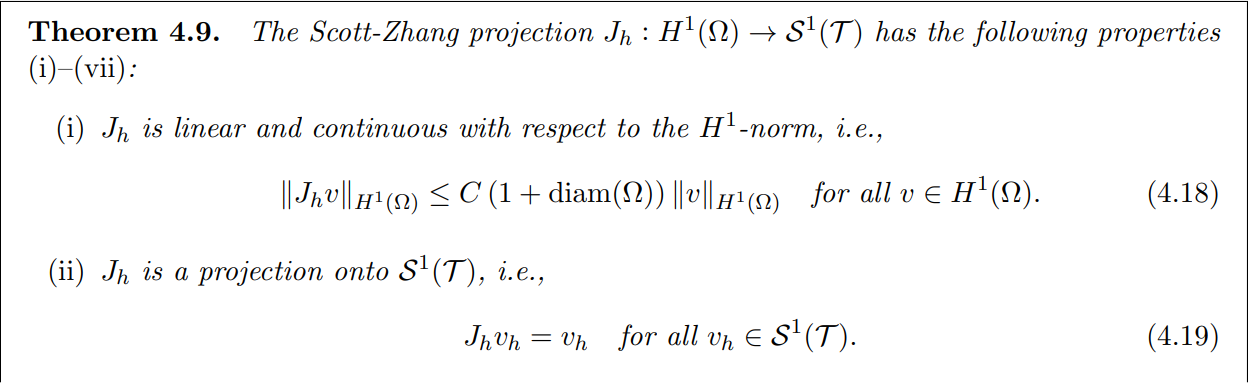
\includegraphics[width = 0.75 \textwidth]{NumPDEs/NumPDEs - Theorem 4.9.1.png} \\
    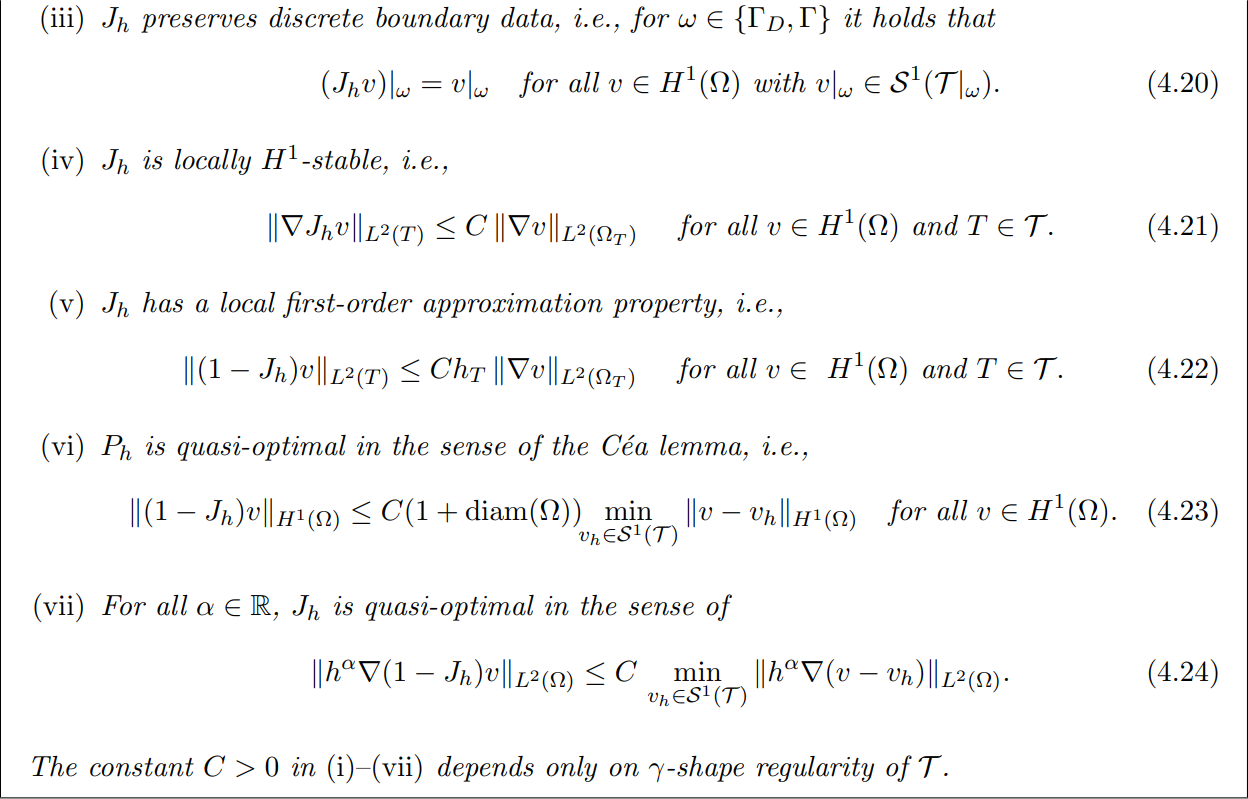
\includegraphics[width = 0.75 \textwidth]{NumPDEs/NumPDEs - Theorem 4.9.2.png}
  \end{tcolorbox}

  \begin{tcolorbox}[standard jigsaw, opacityback = 0]
    \centering
    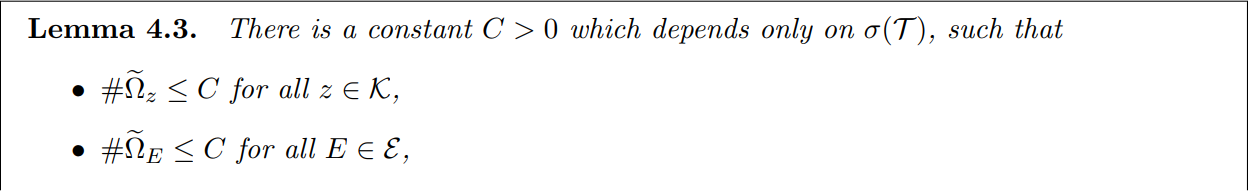
\includegraphics[width = 0.75 \textwidth]{NumPDEs/NumPDEs - Lemma 4.3.1.png} \\
    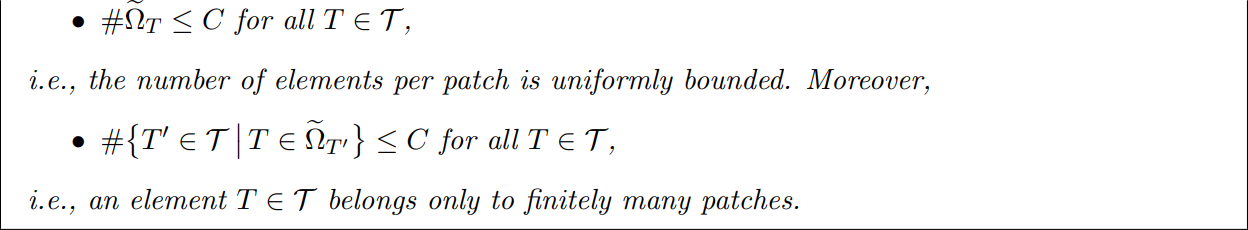
\includegraphics[width = 0.75 \textwidth]{NumPDEs/NumPDEs - Lemma 4.3.2.png}
  \end{tcolorbox}

  Die Approximations-Eigenschaft des Clément-Operators $J_h$, d.h. Lemma 4.9 (v) und der letzte Unterpunkt von Lemma 4.3 implizieren

  \begin{align*}
    & \sum_{T \in \mathcal{T}}
    \norm[L^2(T)]{f - (b \cdot \nabla u_h + c u_h)}
    \norm[L^2(T)]{v - J_h v} \\
    & \stackrel
    {
      \mathrm{4.9 (v)}
    }{\leq}
    \sum_{T \in \mathcal{T}}
    \norm[L^2(T)]{f - (b \cdot \nabla u_h + c u_h)}
    C_1 h_T
    \norm[L^2(\Omega_T)]{\nabla v} \\
    & \stackrel
    {
      \mathrm{CSB}
    }{\leq}
    C_1
    \pbraces
    {
      \sum_{T \in \mathcal{T}}
      \norm[L^2(T)]{h_\mathcal{T} (f - b \cdot \nabla u_h - c u_h)}^2
    }^{1/2}
    \pbraces
    {
      \sum_{T \in \mathcal{T}}
      \norm[L^2(\Omega_T)]{\nabla v}^2
    }^{1/2} \\
    & \stackrel
    {
      \mathrm{4.3}
    }{\leq}
    C_1 C_2
    \pbraces
    {
      \sum_{T \in \mathcal{T}}
      \norm[L^2(T)]{h_\mathcal{T} (f - b \cdot \nabla u_h - c u_h)}^2
    }^{1/2}
    \pbraces
    {
      \sum_{T \in \mathcal{T}}
      \norm[L^2(T)]{\nabla v}^2
    }^{1/2} \\
    & =
    C_1 C_2
    \norm[L^2(\Omega)]{h_\mathcal{T} (f - b \cdot \nabla u_h - c u_h)}
    \norm[L^2(\Omega)]{\nabla v}
  \end{align*}

  Für jede Kante $E \in \mathcal{E}$, wählen wir ein arbiträres Element $T_E \in \mathcal{T}$ mit $E \in \mathcal{E}_{T_E}$.
  Sei $\mathcal{E}_\ast \subset \mathcal{E}$ und $\psi \in L^2(E)$ für alle $E \in \mathcal{E}_\ast$.
  Man erinnere sich an Lemma 4.10.

  \includegraphicsboxed{NumPDEs/NumPDEs - Lemma 4.10.png}

  Daher, zeigen die selben Argumente wie zuvor, dass

  \begin{align*}
    \sum_{E \in \mathcal{E}_\ast}
    \norm[L^2(E)]{\psi}
    \norm[L^2(E)]{v - J_h v}
    & \stackrel
    {
      \mathrm{4.10}
    }{\leq}
    \sum_{E \in \mathcal{E}_\ast}
    \norm[L^2(E)]{\psi}
    C_3 h_E^{1/2}
    \norm[L^2(\Omega_{T_E})]{\nabla v} \\
    & \stackrel
    {
      \mathrm{CSB}
    }{\leq}
    C_3
    \pbraces
    {
      \sum_{E \in \mathcal{E}_\ast}
      \norm[L^2(E)]{h_\mathcal{E}^{1/2} \psi}^2
    }^{1/2}
    \pbraces
    {
      \sum_{E \in \mathcal{E}_\ast}
      \norm[L^2(\Omega_{T_E})]{\nabla v}^2
    }^{1/2} \\
    & \stackrel{!}{\leq}
    C_3
    \pbraces
    {
      \sum_{E \in \mathcal{E}_\ast}
      \norm[L^2(E)]{h_\mathcal{E}^{1/2} \psi}^2
    }^{1/2}
    \pbraces
    {
      3
      \sum_{T \in \mathcal{T}}
      \norm[L^2(T)]{\nabla v}^2
    }^{1/2} \\
    & =
    \sqrt{3} C_3
    \norm[L^2(\mathcal{E}_\ast)]{h_\mathcal{E}^{1/2} \psi}
    \norm[L^2(\Omega)]{\nabla v},
  \end{align*}

  wobei wir bemerken, dass ein Element $T \in \mathcal{T}$ nur $= T_E$ sein kann auf höchstens $3$ Kanten.
  Die Euklid-Norm ist zur Manhattan-Norm auf dem $\R^2$ äquivalent, vermöge $1$ bzw. $\sqrt{2}$.
  Insgesamt sehen wir nun ($\psi := \dbbraces{\partial_n u_h}$ und $\mathcal{E}_\ast := \mathcal{E}_\Omega)$)

  \begin{align*}
    R_h(v)
    & \leq
    C_1 C_2
    \norm[L^2(\Omega)]{h_\mathcal{T} (f - b \cdot \nabla u_h - c u_h)}
    \norm[L^2(\Omega)]{\nabla v}
    +
    \sqrt{3} C_3
    \norm[L^2(\mathcal{E}_\Omega)]{h_\mathcal{E}^{1/2} \dbbraces{\partial_n u_h}}
    \norm[L^2(\Omega)]{\nabla v} \\
    & \leq
    \max \Bbraces{C_1 C_2, \sqrt{3} C_3}
    \norm[L^2(\Omega)]{\nabla v}
    \pbraces
    {
      \norm[L^2(\Omega)]{h_\mathcal{T} (f - b \cdot \nabla u_h - c u_h)}
      +
      \norm[L^2(\mathcal{E}_\Omega)]{h_\mathcal{E}^{1/2} \dbbraces{\partial_n u_h}}
    } \\
    & \leq
    \max \Bbraces{C_1 C_2, \sqrt{3} C_3}
    \norm[L^2(\Omega)]{\nabla v}
    \sqrt{2}
    \pbraces
    {
      \norm[L^2(\Omega)]{h_\mathcal{T} (f - b \cdot \nabla u_h - c u_h)}^2
      +
      \norm[L^2(\mathcal{E}_\Omega)]{h_\mathcal{E}^{1/2} \dbbraces{\partial_n u_h}}^2
    }^{1/2} \\
    & \leq
    \sqrt{2}
    \max \Bbraces{C_1 C_2, \sqrt{3} C_3}
    \norm[L^2(\Omega)]{\nabla v}
    \eta.
  \end{align*}

  Nun gilt es, die Vorbemerkungen des Beweises von dem originalem Theorem 4.11 nachzubauen.
  Weil $v \in \in H_D^1(\Omega)$ beliebig war, folgt

  \begin{align*}
    \implies
    \sup_{w \in H_D^1(\Omega)}
    \frac
    {
      R_h(w)
    }{
      \norm[L^2(\Omega)]{\nabla w}
    }
    \leq
    \sqrt{2}
    \max \Bbraces{C_1 C_2, \sqrt{3} C_3}
    \eta.
  \end{align*}

  Nachdem $u \in H_D^1(\Omega)$ ja eine schwache Lösung ist,

  \begin{align*}
    \implies
    R_h(v)
    =
    F(v) - a(u_h, v)
    =
    \underbrace
    {
      F(v) - a(u, v)
    }_0
    +
    a(u, v)
    -
    a(u_h, v)
    =
    a(u - u_h, v).
  \end{align*}

  Es seien $L$ die Stetigkeits- und $M$ die Elliptizitäts-Konstante von $a$.

  \begin{multline*}
    M \norm[H^1(\Omega)]{u - u_h}
    =
    \frac
    {
      M \norm[H^1(\Omega)]{u - u_h}^2
    }{
      \norm[H^1(\Omega)]{u - u_h}
    }
    \leq
    \frac
    {
      M \norm[H^1(\Omega)]{u - u_h}^2
    }{
      \norm[L^2(\Omega)]{\nabla (u - u_h)}
    }
    \leq
    \frac
    {
      a(u - u_h, u - u_h)
    }{
      \norm[L^2(\Omega)]{\nabla (u - u_h)}
    } \\
    =
    \frac
    {
      R_h(u - u_h)
    }{
      \norm[L^2(\Omega)]{\nabla (u - u_h)}
    }
    \leq
    \sup_{w \in H_D^1(\Omega)}
    \frac
    {
      R_h(w)
    }{
      \norm[L^2(\Omega)]{\nabla w}
    }
  \end{multline*}

  Damit erhalten wir nun endlich unsere finale Abschätzung.

  \begin{align*}
    C
    :=
    \frac
    {
      \sqrt{2}
      \max \Bbraces{C_1 C_2, \sqrt{3} C_3}
    }{
      M
    }
    \implies
    \norm[H^1(\Omega)]{u - u_h}
    \leq
    C \eta
  \end{align*}

  Die (nicht versteckte) Konstante $C$ hängt nur ab (von dem Clemént-Operator $J_h$ und) von der $\gamma$-Form-Regularität von $\mathcal{T}$.

\end{enumerate}

\end{solution}

% --------------------------------------------------------------------------------

% -------------------------------------------------------------------------------- %

\begin{exercise}

Beweisen Sie die Aussage aus Ex. 26 des Vorlesungsskriptes.

\end{exercise}

% -------------------------------------------------------------------------------- %

\begin{solution}

\phantom{}

\end{solution}

% -------------------------------------------------------------------------------- %

% -------------------------------------------------------------------------------- %

\begin{exercise}

Beweisen Sie die Aussagen aus Ex. 29 und Ex. 30 des Vorlesungsskriptes.
\includegraphicsunboxed{NumPDEs/NumPDEs - Exercise 29}
\includegraphicsunboxed{NumPDEs/NumPDEs - Exercise 30}

\end{exercise}

% -------------------------------------------------------------------------------- %

\begin{solution}

\textit{Aufgabe 29.}

Dem Hinweis nach definieren wir

\begin{align*}
  \mathcal{X}_\infty
  :=
  \overline{\bigcup_{\ell=0}^\infty \mathcal{X}_\ell}
  \subset H
\end{align*}

Um die Aussage zu zeigen werden wir nun Proposition $1.7$ benutzen.

\includegraphicsunboxed{NumPDEs/NumPDEs - Proposition 1.7}

Da $\bigcup_{\ell \in \N} \mathcal{X}_\ell$ nach Konstruktion dicht in $\mathcal{X}_\infty$ liegen gilt es also zu zeigen:

\begin{align*}
  \forall v \in \bigcup_{\ell \in \N} \mathcal{X}_\ell: ~
  \lim_{\ell \to \infty} \min_{v_\ell \in \mathcal{X}_\ell}
  \norm[H]{v - v_\ell} = 0
\end{align*}

Sei also $v \in \bigcup_{\ell \in \N} \mathcal{X}_\ell$, dann gilt sicher

\begin{align*}
  \exists k \in \N: v \in \mathcal{X}_k,
\end{align*}

Weil diese Unterräume bezüglich $\subset$ aufsteigend angeordnet sind sogar

\begin{align*}
  \forall \ell \geq k: v \in \mathcal{X}_\ell
\end{align*}

Damit schließen wir, da das Minimum auf einem kleineren Raum stets größer ist

\begin{align*}
  \forall \ell \geq k: \quad
  \min_{v_\ell \in \mathcal{X}_\ell} \norm[H]{v - v_\ell}
  \leq
  \min_{v_k \in \mathcal{X}_k} \norm[H]{v - v_k}
  \leq
  \norm[H]{v-v}
  =
  0
\end{align*}

Da $\mathcal{X}_\infty \supseteq \mathcal{X}_l$ gilt
\begin{align*}
  \forall v \in \mathcal{X}_l: \langle \langle U_\infty; v \rangle \rangle =
  \langle \langle u; v \rangle \rangle
  = \langle \langle \mathbb{G}_l u; v \rangle \rangle
\end{align*}
und es folgt $\mathbb{G}_l(u) = \mathbb{G}_l(U_\infty)$ und es gilt nach Proposition $1.7$:

\begin{align*}
  \lim_{\ell \to \infty} ||U_\infty - \underbrace{\mathbb{G}_\ell U_\infty}_{U_\ell}||_H
  =
  0
\end{align*}

\textit{Aufgabe 30.}

Definieren wir $\mathcal{X}_\infty$ so wie im vorherigen Aufgabenteil. Dann gilt es zu zeigen

\begin{align*}
  \forall u \in H^1_D(\Omega):
  \exists (u_k)_{k \in \N} \in \Big(\bigcup_{\ell \in \N} \mathcal{S}^1_D(\mathcal{T}_\ell)\Big)^\N:
  \quad
  \lim_{k \to \infty} \norm[H^1(\Omega)]{u - u_k} = 0
\end{align*}

Da wir gleichmäßig verfeinern gilt, wenn wir mit $h_0 := \max_{T \in \mathcal{T}_0} \diam T$ bezeichnen

\begin{align*}
  \forall \ell \in \N:~
  h_\ell
  =
  \frac{h_0}{2^\ell}
\end{align*}

Es gilt ebenfalls

\begin{align*}
  \forall \ell \in \N:~
  \sigma(\mathcal{T}_\ell) = \sigma(\mathcal{T}_0)
\end{align*}

Für beliebiges $u \in H^1_D(\Omega) = \overline{C^\infty_D(\overline{\Omega})}^{||\cdot||_{H^1(\Omega)}}$ wollen wir nun wieder Proposition $1.7$ verwenden. Unseren dichten Teilraum für den wir die Approximationseigenschaft zeigen wollen haben wir nun schon bestimmt. Zusätzlich benötigen wir noch Korollar $3.6$ (wobei hier $C^\infty_D(\overline{\Omega}) \subset H^2(\Omega) \cap H^1_D(\Omega)$ mit eingeht).

\includegraphicsunboxed{NumPDEs/NumPDEs - Corollary 3.6}

Sei nun also $v \in C^\infty_D(\overline{\Omega})$, dann erhalten wir

\begin{align*}
  \min_{v_\ell \in \mathcal{S}^1_D(\mathcal{T}_\ell)} \norm[H^1(\Omega)]{v - v_\ell}
  \stackrel{3.6}{\leq}
  C \sigma(\mathcal{T}_\ell)\norm[L^2(\Omega)]{h_\ell D^2v}
  =
  C \sigma(\mathcal{T}_0) \frac{h_0}{2^\ell} \norm[L^2(\Omega)]{D^2v}
  \stackrel{\ell \to \infty}{\longrightarrow}
  0
\end{align*}

Damit gilt nach Proposition $1.7$ nun auch

\begin{align*}
  \lim_{k \to \infty} \|u - \underbrace{\mathbb{G}_ku}_{=:u_k}\|_{H^1(\Omega)} = 0
\end{align*}
\end{solution}

% -------------------------------------------------------------------------------- %

% --------------------------------------------------------------------------------

\begin{exercise}

Sei $u \in H_0^1(\Omega)$ für ein beschränktes Lipschitz-Gebiet $\Omega \subset \R^2$
die Lösung des Poisson-Problems
\begin{align}
  \forall v \in H_0^1(\Omega): (\nabla u;\nabla v)_{L^2(\Omega)} = (f;v)_{L^2(\Omega)}
\end{align}
und $u_h \in \mathcal{S}_0^1(\mathcal{T})$ die zugehörige diskrete Finite-Elemente Lösung.
Weiter sei $\mathcal{K}$ die Knotenmenge der Triangulierung $\mathcal{T}$,
$\zeta_z \in \mathcal{S}_0^1(\mathcal{T})$ für alle $z \in \mathcal{K}$ die Hutfunktionen,
$\tilde{\Omega}_z := \{T \in \mathcal{T}: z \in T\}$ der Knotenpatch aus Abschnitt 4.2 und
\begin{align}
  \tilde{v}_h := \sum_{z \in \mathcal{K}}\left(\frac{1}{|\tilde{\Omega}_z|}
  \sum_{T \in \tilde{\Omega}_z}\nabla u_h|_T\right)\zeta_z
\end{align}
der gemittelte Gradient von $u_h$.
\begin{enumerate}[label = \textbf{\alph*)}]
  \item Beweisen Sie, dass
  \begin{align}
    \eta_{ZZ} := \|\nabla u_h - \tilde{v}_h\|_{L^2(\Omega)}
  \end{align}
  ein zuverlässiger und effizienter Fehlerschätzer ist, wenn der gemittelte
  Gradient eine bessere Approximation an den echten Gradienten ist, als der
  Gradient der FE-Lösung, das heißt, wenn eine Konstante $\alpha < 1$ existiert,
  sodass
  \begin{align}
    \|\nabla u - \tilde{v}_h\|_{L^2(\Omega)} \leq \alpha\|\nabla u - \nabla u_h\|_{L^2(\Omega)}.
    \label{ineq_grad}
  \end{align}
  \item Implementieren Sie diesen Fehlerschätzer in NGSolve und testen Sie numerisch
  sowohl die Güte des Fehlerschätzers als auch die Ungleichung \eqref{ineq_grad}.
  Konstruieren Sie sich dazu analog zu Beispiel 10 geeignete Referenzlösungen. \\

  \textit{Hinweis:} In NGSolve ist $\tilde{v}_h$ sehr elegant mit den Code-Zeilen
  \begin{itemize}
    \item $\mathrm{fe\_ag = VectorH1(mesh, order = 1)}$
    \item $\mathrm{vtilde = GridFunction(fe\_ag)}$
    \item $\mathrm{flux = grad(gfu)}$
    \item $\mathrm{vtilde.Set(flux)}$
  \end{itemize}
  zu berechnen.
\end{enumerate}
\end{exercise}

% --------------------------------------------------------------------------------

\begin{solution}

\begin{enumerate}[label = \textbf{\alph*)}]
  \item Erinnern wir uns daran, was es heißt zuverlässig und effizient zu sein. Es gilt zu zeigen

  \begin{align*}
    \norm[H^1(\Omega)]{u - u_h} &\leq C_{\text{rel}}~ \eta_{ZZ} \\
    C_{\text{eff}}~ \eta_{ZZ} &\leq \norm[H^1(\Omega)]{u - u_h}
  \end{align*}

  Um die Effizienz zu zeigen können wir \ref{ineq_grad} direkt verwenden:

  \begin{align*}
    \eta_{ZZ}
    &=
    \norm[L^2(\Omega)]{\nabla u_h - \tilde{v}_h}
    \leq
    \norm[L^2(\Omega)]{\nabla u - \nabla u_h} + \norm[L^2(\Omega)]{\nabla u - \tilde{v}_h}
    \stackrel{\ref{ineq_grad}}{\leq}
    (1 + \alpha) \norm[L^2(\Omega)]{\nabla u - \nabla u_h} \\
    &\leq
    (1 + \alpha) \norm[H^1(\Omega)]{u - u_h}
  \end{align*}

  Für die Zuverlässigkeit multiplizieren wir \ref{ineq_grad} mit $-1$ und sehen dadurch

  \begin{align*}
    \norm[L^2(\Omega)]{\nabla u - \nabla u_h} - \norm[L^2(\Omega)]{\nabla u - \tilde{v}_h}
    \geq
    (1 - \alpha) \norm[L^2(\Omega)]{\nabla u - \nabla u_h}
  \end{align*}

  Damit, sowie mit der Poincare-Ungleichung schätzen wir nun ab:
  \includegraphicsboxed{PDEs/PDEs_-_Satz_5-11_(Poincare-Ungleichung)}
  \begin{align*}
    \norm[H^1{\Omega}]{u - u_h}
    &=
    \sqrt{\norm[L^2(\Omega)]{u - u_h}^2 + \norm[L^2(\Omega)]{\nabla u - \nabla u_h}^2}
    \leq
    \underbrace{\sqrt{(1+C_p^2)}}_{:=C} \norm[L^2(\Omega)]{\nabla u - \nabla u_h} \\
    &\leq
    \frac{C}{1-\alpha} \Big(
      \norm[L^2(\Omega)]{\nabla u - \nabla u_h} - \norm[L^2(\Omega)]{\nabla u - \tilde{v}_h}
    \Big) \\
    &\leq
    \frac{C}{1-\alpha} \Big(
      \norm[L^2(\Omega)]{\nabla u - \tilde{v}_h} + \norm[L^2(\Omega)]{\nabla u_h - \tilde{v}_h} - \norm[L^2(\Omega)]{\nabla u - \tilde{v}_h}
      \Big)
    =
    \frac{C}{1-\alpha} \eta_{ZZ}
  \end{align*}

  \item Siehe ipynb-File.
\end{enumerate}

\end{solution}

% --------------------------------------------------------------------------------

% --------------------------------------------------------------------------------

\begin{exercise}

Lösen Sie die Rekursion $T(1) = 1$ und $T(n) = 3T(\frac{n}{2}) + n^2 + n$ für $n = 2^k \geq 2$, indem Sie wiederholt in die Rekursion einsetzen, bis Sie $T(n)$ erkennen. Verifizieren Sie ihr Ergebnis anschließend mit der Substitutionsmethode.

\end{exercise}

% --------------------------------------------------------------------------------

\begin{solution}

Setzen wir also zuerst ein paar mal ein (und addieren dabei nicht direkt damit man das Schema erkennen kann):

\begin{align*}
  T(2^0) &= 1 \\
  T(2^1) &= 3 + 4 + 2 = 2 + 3 + 2^2 \\
  T(2^2) &= 3\cdot2 + 3^2 +3\cdot2^2 + 2^4 + 2^2 = 2^2 + 2\cdot3 + 3^2+ 2^4+ 3\cdot2^2\\
  T(2^3) &= 3^2\cdot2 + 3^3 +2^2\cdot3^2 +3\cdot2^4 +3\cdot2^2 + 2^6 +2^3 = 2^3 + 2^2\cdot3 + 2\cdot3^2 + 3^3 + 2^4+ 2^6 +3\cdot2^4 + 3^2\cdot2^2
\end{align*}

Wir stellen die Vermutung

\begin{align*}
  T(2^k) = \sum_{i=0}^k 2^{k-i}3^i + \sum_{i=0}^{k-1} 2^{2(k-i)} 3^i
\end{align*}
auf. Um diese zu Verifizieren verwenden wir Induktion (über $k$). \\
IA$(k=0)$:

\begin{align*}
  T(1) = 1 = 2^0 \cdot 3^0
\end{align*}
IV: $T(2^k) = \sum_{i=0}^k 2^{k-i}3^i + \sum_{i=0}^{k-1} 2^{2(k-i)} 3^i$ \\

IS:~$k \mapsto k+1$
\begin{align*}
  T(2^{k+1})
  &=
  3T(2^k) + 2^{2(k+1)} + 2^{k+1}
  \stackrel{IV}{=}
  3(\sum_{i=0}^k 2^{k-i}3^i + \sum_{i=0}^{k-1} 2^{2(k-i)} 3^i) + 2^{2(k+1)} + 2^{k+1} \\
  &=
  \sum_{i=0}^k 2^{k-i}3^{i+1} + \sum_{i=0}^{k-1} 2^{2(k-i)} 3^{i+1} + 2^{2(k+1)} + 2^{k+1}
  =
  \sum_{i=1}^{k+1} 2^{k-(i-1)}3^{i} + \sum_{i=1}^{k} 2^{2[k-(i-1)]} 3^{i} + 2^{2(k+1)} + 2^{k+1} \\
  &=
  \sum_{i=0}^{k+1} 2^{k+1-i}3^{i} + \sum_{i=0}^{k} 2^{2[(k+1)-i]} 3^{i}
\end{align*}

\end{solution}

% --------------------------------------------------------------------------------


\printbibliography

\end{document}
